\documentclass{article}
\usepackage{tikz}
\begin{document}


\thispagestyle{empty}
\begin{center}
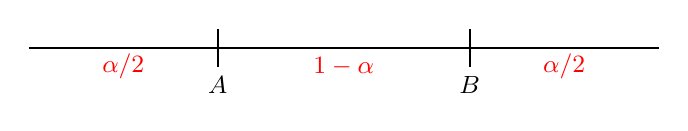
\begin{tikzpicture}[thick,scale=0.8]%[>=stealth]%,yscale=0.5,xscale=0.7]
\draw (0,0)--(10,0);
\draw (3,0.3)--(3,-0.3);
\draw (7,0.3)--(7,-0.3);
\draw(3,-0.6) node {\small $A$}; 
\draw (7,-0.6) node {\small $B$}; 
\draw[red] (8.5,-0.3) node {\small $\alpha/2$}; 
\draw[red] (1.5,-0.3) node {\small $\alpha/2$}; 
\draw[red] (5,-0.3) node {\small $1-\alpha$}; 
\end{tikzpicture}
\end{center}

\end{document}